\appendix
\chapter{Preferred Direction Diffusion Scheme}
This chapter provides a detailed derivation of the integral calculations to obtain the coefficients in (\ref{eq:a21}).
\label{app:aa}
\section{Cell Properties}
\label{sec:one}
\begin{comment}
\begin{figure}[H]
\centering
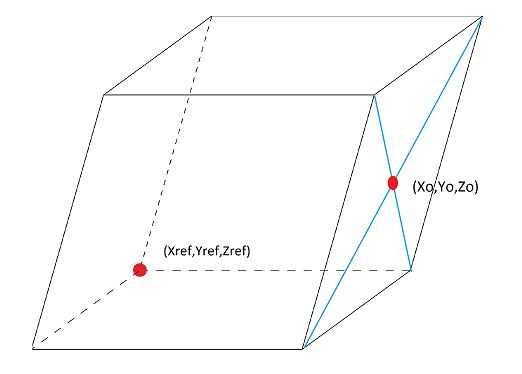
\includegraphics[scale=0.6]{include/backmatter/cdd.JPG}
\caption{Representation of a cell in Physical Space}
\label{fig:cellp}
\end{figure}
\end{comment}
Twenty cell properties are calculated for each cell using an uniquely defined reference node point $(x_{ref},y_{ref},z_{ref})$ .
\begin{equation}\label{eq:eqns}
\begin{gathered}
\nonumber
\mathcal{V}_{o_k}=\int\int\int_{\Omega_k}d\Omega \\
\mathcal{V}_{x_k}=\int\int\int_{\Omega_k}(x-x_{ref})d\Omega\\ 
\mathcal{V}_{y_k}=\int\int\int_{\Omega_k}(y-y_{ref})d\Omega\\ 
\mathcal{V}_{z_k}=\int\int\int_{\Omega_k}(z-z_{ref})d\Omega\\ 
\mathcal{V}_{xx_k}=\int\int\int_{\Omega_k}(x-x_{ref})^2d\Omega\\ 
\mathcal{V}_{xy_k}=\int\int\int_{\Omega_k}(x-x_{ref})(y-y_{ref})d\Omega\\ 
\mathcal{V}_{xz_k}=\int\int\int_{\Omega_k}(x-x_{ref})(z-z_{ref})d\Omega\\ 
\mathcal{V}_{yy_k}=\int\int\int_{\Omega_k}(y-y_{ref})^2d\Omega\\ 
\mathcal{V}_{yz_k}=\int\int\int_{\Omega_k}(y-y_{ref})(z-z_{ref})d\Omega\\ 
\mathcal{V}_{zz_k}=\int\int\int_{\Omega_k}(z-z_{ref})^2d\Omega\\ 
\mathcal{V}_{xxx_k}=\int\int\int_{\Omega_k}(x-x_{ref})^3d\Omega\\ 
\mathcal{V}_{xxy_k}=\int\int\int_{\Omega_k}(x-x_{ref})^2(y-y_{ref})d\Omega\\ 
\mathcal{V}_{xxz_k}=\int\int\int_{\Omega_k}(x-x_{ref})^2(z-z_{ref})d\Omega\\ 
\mathcal{V}_{xyy_k}=\int\int\int_{\Omega_k}(x-x_{ref})(y-y_{ref})^2d\Omega\\ 
\frac{\partial (\rho k)}{\partial t}+\frac{\partial (\rho k <V_j>)}{\partial x_j}=P_k-\beta^*k w+\frac{\partial}{\partial x_j}(\Gamma_{k}\frac{\partial k}{\partial x_j})\\
\frac{\partial (\rho \omega)}{\partial t}+\frac{\partial (\rho \omega <V_j>)}{\partial x_j}=\frac{\gamma}{\nu}P_k-\beta\rho\omega^2+\frac{\partial}{\partial x_j}(\Gamma_{\omega}\frac{\partial \omega}{\partial x_j})+2(1-F_1)\sigma_{w2}\frac{1}{\omega}\frac{\partial k}{\partial x_j}\frac{\partial \omega}{\partial x_j}
\end{gathered}
\end{equation}\\
\begin{equation}\label{fig:other}
\begin{gathered}
\mathcal{V}_{xyz_k}=\int\int\int_{\Omega_k}(x-x_{ref})(y-y_{ref})(z-z_{ref})d\Omega\\ 
\mathcal{V}_{xzz_k}=\int\int\int_{\Omega_k}(x-x_{ref})(z-z_{ref})^2d\Omega\\ 
\mathcal{V}_{yyy_k}=\int\int\int_{\Omega_k}(y-y_{ref})^3d\Omega\\ 
\mathcal{V}_{yyz_k}=\int\int\int_{\Omega_k}(y-y_{ref})^2(z-z_{ref})d\Omega\\ 
\mathcal{V}_{yzz_k}=\int\int\int_{\Omega_k}(y-y_{ref})(z-z_{ref})^2d\Omega\\ 
\mathcal{V}_{zzz_k}=\int\int\int_{\Omega_k}(z-z_{ref})^3d\Omega\\
\frac{\partial (\rho k)}{\partial t}+\frac{\partial (\rho k <V_j>)}{\partial x_j}=P_k-\beta^*k w+\frac{\partial}{\partial x_j}(\Gamma_{k}\frac{\partial k}{\partial x_j})
\frac{\partial (\rho \omega)}{\partial t}+\frac{\partial (\rho \omega <V_j>)}{\partial x_j}=\frac{\gamma}{\nu}P_k-\beta\rho\omega^2+\frac{\partial}{\partial x_j}(\Gamma_{\omega}\frac{\partial \omega}{\partial x_j})+2(1-F_1)\sigma_{w2}\frac{1}{\omega}\frac{\partial k}{\partial x_j}\frac{\partial \omega}{\partial x_j}
 \end{gathered}
\end{equation}
\section*{Tri-Linear Parametrization}
The Cell properties in \ref{sec:one} are calculated for each of the ten cells per face using Gauss-point Quadrature. Initially a local coordinate system $(x',y',z')$ is defined for each cell. This system with respect to the global co-ordinate system is obtained using tri-linear parametrization. 
\begin{figure}[h]
\centering
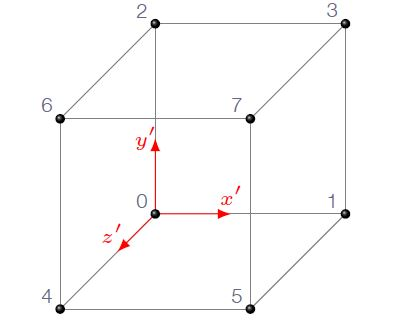
\includegraphics[height=8cm]{include/backmatter/tlp.JPG}
\caption{Representation of local co-ordinate sytem of a cell in physical space }
\label{fig:tlpcell}
\end{figure}
\begin{equation}\label{eq:tlm}
 \begin{gathered}
 x=(1-x')(1-y')(1-z')x_0+x'(1-y')(1-z')x_1+\\
 (1-x')y'(1-z')x_2+x'y'(1-z')x_3+(1-x')(1-y')z'x_4+\\
 x'(1-y')z'x_5+(1-x')y'z'x_6+x'y'z'x_7 \\
 y=(1-x')(1-y')(1-z')y_0+x'(1-y')(1-z')y_1+\\
 (1-x')y'(1-z')y_2+x'y'(1-z')y_3+(1-x')(1-y')z'y_4+\\
 x'(1-y')z'y_5+(1-x')y'z'y_6+x'y'z'y_7 \\
 z=(1-x')(1-y')(1-z')z_0+x'(1-y')(1-z')z_1+\\
 (1-x')y'(1-z')z_2+x'y'(1-z')z_3+(1-x')(1-y')z'z_4+\\
 x'(1-y')z'z_5+(1-x')y'z'z_6+x'y'z'z_7 \\
 \end{gathered}
 \end{equation}
 \section*{Gauss-point Quadrature}\label{sec:gpq}
 Using the equations in (\ref{eq:tlm}), the volume integrals in (\ref{eq:eqns}) are calculated using Gauss-point Quadrature numerical integration method. The general representation of the integration is given by,
 \begin{equation}
 \begin{gathered}
     \label{eq:gauss}
     \int\int\int_{\Omega_k} \phi(x,y,z) \,dxdydz=\int_{0}^{1}\int_{0}^{1}\int_{0}^{1}\phi(x',y',z')J\,dx'dy'dz'\\
     $where Jacobian J is defined as,$\\
     \begin{vmatrix}
    \frac{\partial x}{\partial x'} & \frac{\partial x}{\partial y'} & \frac{\partial x}{\partial z'}\\
    \frac{\partial y}{\partial x'} & \frac{\partial y}{\partial y'} & \frac{\partial y}{\partial z'}\\
    \frac{\partial z}{\partial x'} & \frac{\partial z}{\partial y'} & \frac{\partial z}{\partial z'}
    \end{vmatrix}
     \end{gathered}
 \end{equation}
 In order to use the Gauss-point quadrature, the range of the local coordinate system must be redefined from -1 to 1.
 \begin{equation}
 \begin{gathered}
     \label{eq:gaussfinal}
     \int\int\int_{\Omega_k} \phi(x,y,z)\,dxdydz=\frac{1}{8}\int_{-1}^{1}\int_{-1}^{1}\int_{-1}^{1}\phi(x'',y'',z'')J(x'',y'',z'')\,dx''dy''dz''
     \end{gathered}
     \end{equation}
     \begin{equation}
     \label{eq:gaussfinal2}
     \int\int\int_{\Omega_k} \phi(x,y,z)\,dxdydz=\frac{1}{8}\sum\limits_{i=1}^{n}\sum\limits_{j=1}^{n}\sum\limits_{k=1}^{n}w_iw_jw_k\phi(p_i,p_j,p_k)J(p_i,p_j,p_k)
     \end{equation}
     Where $p_i,p_j,p_k$ are the Gauss points and $w_i,w_j,w_k$ are the corresponding weights.
     
    
\section*{Volume Integrals}\label{sec:vi}
The integrals in matrix $A$ is calculated using the relationship between the $(\xi,\eta,\zeta)$ space and $(x,y,z)$ space in (\ref{eq:lcs}).
\begin{equation}
    \label{eq:a11}
    \begin{gathered}
    \xi=\Psi_{11}(x-x_o)+\Psi_{12}(y-y_o)+\Psi_{13}(z-z_o)\\
    \eta=\Psi_{21}(x-x_o)+\Psi_{22}(y-y_o)+\Psi_{23}(z-z_o)\\
    \zeta=\Psi_{31}(x-x_o)+\Psi_{32}(y-y_o)+\Psi_{33}(z-z_o)\\
    \end{gathered}
\end{equation}
The following relations are used to rewrite the integrals,
\begin{equation}
    \label{eq:a12}
    \begin{gathered}
    (x-x_o)=((x-x_{ref})+(x_{ref}-x_o))\\
    (y-y_o)=((y-y_{ref})+(y_{ref}-y_o))\\
    (z-z_o)=((z-z_{ref})+(z_{ref}-z_o))\\
    \end{gathered}
\end{equation}
Introducing the constansts $\Delta x,\Delta y,\Delta z$,
\begin{equation}
    \label{eq:a13}
    \begin{gathered}
    \Delta x=x_{ref}-x_o\\
    \Delta y=y_{ref}-y_o\\
    \Delta z=z_{ref}-z_o\\
    \end{gathered}
\end{equation}
which results in,
\begin{equation}
    \label{eq:a14}
    \begin{gathered}
    (x-x_o)=((x-x_{ref})+\Delta x)\\
    (y-y_o)=((y-y_{ref})+\Delta y)\\
    (z-z_o)=((z-z_{ref})+\Delta z)\\
    \end{gathered}
\end{equation}
The terms in the first column are obtained using the volume integrals in equations (\ref{eq:eqns}). Further, the second, third and fourth columns which consists of first order terms are obtained using the direct relations from equations (\ref{eq:a11}-\ref{eq:a14}).
\begin{equation}
    \label{eq:a15}
    \begin{gathered}
    \int\int\int_{\Omega_k}\xi\,d\Omega=\Psi_{11}(\mathcal{V}_{x_k}+\Delta x\mathcal{V}_{o_k})+\Psi_{12}(\mathcal{V}_{y_k}+\Delta y\mathcal{V}_{o_k})+\Psi_{13}(\mathcal{V}_{z_k}+\Delta z\mathcal{V}_{o_k})\\
    \int\int\int_{\Omega_k}\eta\,d\Omega=\Psi_{21}(\mathcal{V}_{x_k}+\Delta x\mathcal{V}_{o_k})+\Psi_{22}(\mathcal{V}_{y_k}+\Delta y\mathcal{V}_{o_k})+\Psi_{23}(\mathcal{V}_{z_k}+\Delta z\mathcal{V}_{o_k})\\
    \int\int\int_{\Omega_k}\zeta\,d\Omega=\Psi_{31}(\mathcal{V}_{x_k}+\Delta x\mathcal{V}_{o_k})+\Psi_{32}(\mathcal{V}_{y_k}+\Delta y\mathcal{V}_{o_k})+\Psi_{33}(\mathcal{V}_{z_k}+\Delta z\mathcal{V}_{o_k})\\
    \end{gathered}
\end{equation}
Further, the quadratic and cubic terms in matrix $A$ are calculated by rewriting and expanding the products of $\xi$, $\eta$ and $\zeta$.
\begin{equation}
    \label{eq:a16}
    \begin{gathered}
    \xi\eta=\Psi_{11}\Psi_{21}(x-x_o)^2+(\Psi_{11}\Psi_{22}+\Psi_{12}\Psi_{21})(x-x_o)(y-y_o)+\\
    (\Psi_{11}\Psi_{23}+\Psi_{13}\Psi_{21})(x-x_o)(z-z_o)+\Psi_{12}\Psi_{22}(y-y_o)^2+\\
    (\Psi_{12}\Psi_{23}+\Psi_{13}\Psi_{22}(y-y_o)(z-z_o)+\Psi_{13}\Psi_{23}(z-z_o)^2\\
    \xi\zeta=\Psi_{11}\Psi_{31}(x-x_o)^2+(\Psi_{11}\Psi_{32}+\Psi_{12}\Psi_{31})(x-x_o)(y-y_o)+\\
    (\Psi_{11}\Psi_{33}+\Psi_{13}\Psi_{31})(x-x_o)(z-z_o)+\Psi_{12}\Psi_{32}(y-y_o)^2+\\
    (\Psi_{12}\Psi_{33}+\Psi_{13}\Psi_{32}(y-y_o)(z-z_o)+\Psi_{13}\Psi_{33}(z-z_o)^2\\
    \\
    \zeta^2=\Psi_{21}\Psi_{21}(x-x_o)^2+2\Psi_{21}\Psi_{22}(x-x_o)(y-y_o)+\\
    2\Psi_{21}\Psi_{23}(x-x_o)(z-z_o)+\Psi_{22}\Psi_{22}(y-y_o)^2+\\
    2\Psi_{22}\Psi_{23}(y-y_o)(z-z_o)+\Psi_{23}\Psi_{23}(z-z_o)^2\\
    \eta^2=\Psi_{31}\Psi_{31}(x-x_o)^2+2\Psi_{31}\Psi_{32}(x-x_o)(y-y_o)+\\
    2\Psi_{31}\Psi_{33}(x-x_o)(z-z_o)+\Psi_{32}\Psi_{32}(y-y_o)^2+\\
    2\Psi_{32}\Psi_{33}(y-y_o)(z-z_o)+\Psi_{33}\Psi_{33}(z-z_o)^2\\
    \\
    \xi\eta^2=\Psi_{11}\Psi_{21}\Psi_{21}(x-x_o)^3+\\
    (2\Psi_{11}\Psi_{21}\Psi_{22}+\Psi_{12}\Psi_{21}\Psi_{21})(x-x_o)^2(y-y_o)+\\
    (2\Psi_{11}\Psi_{21}\Psi_{23}+\Psi_{13}\Psi_{21}\Psi_{21})(x-x_o)^2(z-z_o)+\\
    (\Psi_{11}\Psi_{22}\Psi_{22}+2\Psi_{12}\Psi_{21}\Psi_{22})(x-x_o)(y-y_o)^2+\\
    (2\Psi_{11}\Psi_{22}\Psi_{23}+2\Psi_{12}\Psi_{21}\Psi_{23}+2\Psi_{13}\Psi_{21}\Psi_{22})\\
    (x-x_o)(y-y_o)(z-z_o)+\\
    (\Psi_{11}\Psi_{23}\Psi_{23}+2\Psi_{13}\Psi_{21}\Psi_{23})(x-x_o)(z-z_o)^2+\\
    \Psi_{12}\Psi_{22}\Psi_{22}(y-y_o)^3+\\
    (2\Psi_{12}\Psi_{22}\Psi_{23}+\Psi_{13}\Psi_{22}\Psi_{22})(y-y_o)^2(z-z_o)+\\
    (\Psi_{12}\Psi_{23}\Psi_{23}+2\Psi_{13}\Psi_{22}\Psi_{23})(y-y_o)(z-z_o)^2+\\
    \Psi_{13}\Psi_{23}\Psi_{23}(z-z_o)^3\\
    \xi\zeta^2=\Psi_{11}\Psi_{31}\Psi_{31}(x-x_o)^3+\\
    (2\Psi_{11}\Psi_{31}\Psi_{32}+\Psi_{12}\Psi_{31}\Psi_{31})(x-x_o)^2(y-y_o)+\\
    (2\Psi_{11}\Psi_{31}\Psi_{33}+\Psi_{13}\Psi_{31}\Psi_{31})(x-x_o)^2(z-z_o)+\\
    (\Psi_{11}\Psi_{32}\Psi_{32}+2\Psi_{12}\Psi_{31}\Psi_{32})(x-x_o)(y-y_o)^2+\\
    (2\Psi_{11}\Psi_{32}\Psi_{33}+2\Psi_{12}\Psi_{31}\Psi_{33}+2\Psi_{13}\Psi_{31}\Psi_{32})\\
    (x-x_o)(y-y_o)(z-z_o)+\\
    (\Psi_{11}\Psi_{33}\Psi_{33}+2\Psi_{13}\Psi_{31}\Psi_{33})(x-x_o)(z-z_o)^2+\\
    \Psi_{12}\Psi_{32}\Psi_{32}(y-y_o)^3+\\
    (2\Psi_{12}\Psi_{32}\Psi_{33}+\Psi_{13}\Psi_{32}\Psi_{32})(y-y_o)^2(z-z_o)+\\
    (\Psi_{12}\Psi_{33}\Psi_{33}+2\Psi_{13}\Psi_{32}\Psi_{33})(y-y_o)(z-z_o)^2+\\
    \Psi_{13}\Psi_{33}\Psi_{33}(z-z_o)^3\\
    \end{gathered}
\end{equation}
Further, the unknown products of $(x-x_o)$, $(y-y_o)$ and $(z-z_o)$ in equations (\ref{eq:a16}) are obtained by expanding and rewriting them using equation (\ref{eq:a14}).
\begin{equation}
    \label{eq:a17}
    \begin{gathered}
    \nonumber
    (x-x_o)^2=(x-x_{ref})^2+2\Delta x(x-x_{ref})+\Delta x^2\\
    \\
    (x-x_o)(y-y_o)=(x-x_{ref})(y-y_{ref})+\\\Delta y(x-x_{ref})+\Delta x(y-y_{ref})+\Delta x\Delta y\\
    \\
    (x-x_o)(z-z_o)=(x-x_{ref})(z-z_{ref})+\\\Delta z(x-x_{ref})+\Delta x(z-z_{ref})+\Delta x\Delta z\\
    \\
    (y-y_o)^2=(y-y_{ref})^2+2\Delta y(y-y_{ref})+\Delta y^2\\
    \\
    (y-y_o)(z-z_o)=(y-y_{ref})(z-z_{ref})+\\\Delta z(y-y_{ref})+\Delta y(z-z_{ref})+\Delta y\Delta z\\
    \\
    (z-z_o)^2=(z-z_{ref})^2+2\Delta z(z-z_{ref})+\Delta z^2\\
    \\
    (x-x_o)^3=(x-x_{ref})^3+3\Delta x(x-x_{ref})^2+\\3\Delta x^2(x-x_{ref})+\Delta x^3\\
    \\
    (x-x_o)^2(y-y_o)=(x-x_{ref})^2(y-y_{ref})+\\2\Delta x(x-x_{ref})(y-y_{ref})+\\
    \Delta x^2(y-y_{ref})+\Delta y(x-x_{ref})^2+\\2\Delta x\Delta y(x-x_{ref})+\Delta x^2\Delta y^2\\
    \\
    (x-x_o)^2(z-z_o)=(x-x_{ref})^2(z-z_{ref})+\\2\Delta x(x-x_{ref})(z-z_{ref})+\\
    \Delta x^2(z-z_{ref})+\Delta z(x-x_{ref})^2+2\Delta x\Delta z(x-x_{ref})+\Delta x^2\Delta z^2\\
    \\
    (x-x_o)(y-y_o)^2=(x-x_{ref})(y-y_{ref})^2+\\2\Delta y(x-x_{ref})(y-y_{ref})+\\
    \Delta y^2 (x-x_{ref})+\Delta x (y-y_{ref})^2+\\2\Delta x\Delta y(y-y_{ref})+\Delta x \Delta y^2\\
    \\
    (x-x_o)(z-z_o)^2=(x-x_{ref})(z-z_{ref})^2+\\2\Delta z(x-x_{ref})(z-z_{ref})+\\
    \Delta z^2 (x-x_{ref})+\Delta x (z-z_{ref})^2+\\2\Delta x\Delta z(z-z_{ref})+\Delta x \Delta z^2\\
    \\
     \end{gathered}
\end{equation}\\
\begin{equation}
\begin{gathered}
\label{eq:dfdf}
    (y-y_o)^3=(y-y_{ref})^3+3\Delta y(y-y_{ref})^2+3\Delta y^2(y-y_{ref})+\Delta y^3\\
    \\
    (y-y_o)^2(z-z_o)=(y-y_{ref})^2(z-z_{ref})+\\2\Delta y(y-y_{ref})(z-z_{ref})+\\
    \Delta y^2(z-z_{ref})+\Delta z(y-y_{ref})^2+\\2\Delta y\Delta z(y-y_{ref})+\Delta y^2\Delta z^2\\
    \\
    (y-y_o)(z-z_o)^2=(y-y_{ref})(z-z_{ref})^2+\\2\Delta z(y-y_{ref})(z-z_{ref})+\\
    \Delta z^2 (y-y_{ref})+\Delta y (z-z_{ref})^2+\\2\Delta y\Delta z(z-z_{ref})+\Delta y \Delta z^2\\
    \\
    (z-z_o)^3=(z-z_{ref})^3+3\Delta z(z-z_{ref})^2+\\3\Delta z^2(z-z_{ref})+\Delta z^3\\
    \\
  (x-x_o)(y-y_o)(z-z_o)=(x-x_{ref})(y-y_{ref})(z-z_{ref})+\\
    \Delta y(x-x_{ref})(z-z_{ref})+\\
    \Delta x(y-y_{ref})(z-z_{ref})+\\\Delta x\Delta y(z-z_{ref})+\\
    \Delta z(x-x_{ref})(y-y_{ref})+\\\Delta y\Delta z(x-x_{ref})+\\
    \Delta x\Delta z(y-y_{ref})+\Delta x\Delta y\Delta z
 \end{gathered}
\end{equation}\\   
Using equations in (\ref{eq:a16} and \ref{eq:dfdf}) together with the cell properties, the quadratic and cubic terms of matrix $A$ can be calculated.

\newpage
\section*{Domain Boundaries}
\begin{figure}[H]
\centering
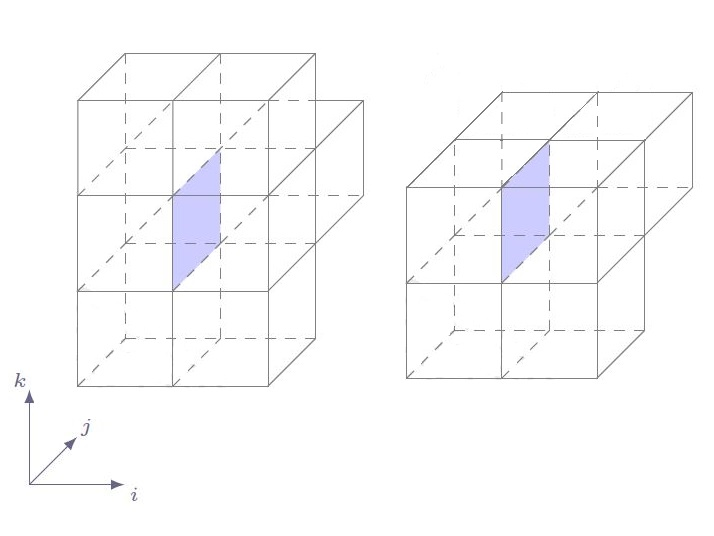
\includegraphics[scale=0.7]{include/backmatter/bd.JPG}
\caption{Representation of Domain Boundaries}
\label{fig:cellb}
\end{figure}
The cell faces present along the domain boundaries do not have ten cells surrounding them. Therefore a truncated flux molecule is considered for the analysis in these cases. A general description of the treatment which is analogous for flux molecules in other directions is discussed below.
\\The first case consists of eight cells with two missing in $\eta$ direction. This reflects in the removal of the terms which includes $\eta^2$ from the equation (\ref{eq:nmnm}). Analogous to this case, the terms containing $\zeta^2$ are removed in the other direction.
\begin{equation}
    {\varphi}(\xi,\eta,\zeta)=C_0+C_1\xi+C_2\eta+C_3\zeta+C_4\xi\eta+C_5\xi\zeta+C_6\zeta^2+C_7\xi\zeta^2
\end{equation}
The second case consists of six cells with two missing in $\eta$ and $\zeta$ directions. This reflects in the removal of the terms which includes $\eta^2$ and $\zeta^2$ from the equation (\ref{eq:nmnm}).
\begin{equation}
    {\varphi}(\xi,\eta,\zeta)=C_0+C_1\xi+C_2\eta+C_3\zeta+C_4\xi\eta+C_5\xi\zeta
\end{equation}



\chapter{Analytical Solution}
\label{app:bb}

This section provides a detailed derivation of the analytical solution for the considered geometry in this project.
The Governing Equation solved here is a 2D Unsteady heat Conduction equation in Cylindrical Coordinate system.
\begin{equation}
    \label{eq:b1}
    \frac{\partial T}{\partial t} = \alpha (\frac{\partial^2 T}{\partial r^2}+\frac{1}{r}\frac{\partial T}{\partial r}+\frac{1}{r^2}\frac{\partial^2 T}{\partial \Theta^2})
\end{equation}
The initial and Boundary conditions are,
\begin{equation}
    \label{eq:b2}
    \begin{gathered}
    T(r=a=1m)=0 \hspace{4cm}T(r=b=1.5m)=0\\
    T(\Theta=0)=0 \hspace{4cm}T(\Theta=\frac{\pi}{2})=0\\
    T(t=0)=F(r,\Theta)=30K
    \end{gathered}
\end{equation}
Using Separation of Variables method of solving Partial Differential Equations,
\begin{equation}
    \label{eq:b3}
    \begin{gathered}
    $let$ \hspace{1cm}T(t,\Theta,t)=R(r).\chi(\Theta).\Gamma(t)\\
    $substituting in (\ref{eq:b1}) results in,$\\
    \frac{1}{R}[R''+\frac{1}{r}R']+\frac{1}{r^2\chi}\chi''=\frac{1}{\alpha\Gamma}\frac{\partial \Gamma}{\partial t}=-\lambda^2
    \end{gathered}
\end{equation}
The general solution of the unsteady term in (\ref{eq:b3}) results in,
\begin{equation}
    \label{eq:b4}
    \Gamma(t)=C_1.e^{-\alpha {\lambda^2} t}
\end{equation}
Further, the general solution of the $\chi$ is obtained as,
\begin{equation}
    \label{eq:b5}
    \begin{gathered}
    \chi(\Theta)=C_2cos(\nu\Theta)+C_3sin(\nu\Theta)\\
    $Applying Boundary conditions,$\\
    \chi(\Theta=0)=0=C_2\\
    \chi(\Theta=\frac{\pi}{2})=0=C_3sin(\nu\frac{\pi}{2})\\
    \nu_n=2n\hspace{0.5cm} n=1,2,3...\\
    \end{gathered}
\end{equation}

Here $\nu_n$ are the Eigen values. Further, the general equation for the $R$ term is obtained as,
\begin{equation}
    \label{eq:b6}
    \begin{gathered}
    R''+\frac{1}{r}R'+(\lambda^2-\frac{\nu^2}{r^2})R=0
    \\
    R(r)=C_4J_\nu(\lambda r)+C_5 Y_\nu(\lambda r)\\
    \\
    $Here $J_\nu$ and $Y_\nu$ are Bessel functions of the first and second order respectively.$\\
    $Further, applying the Boundary conditions,$\\
    R(a)=0=C_4J_\nu(\lambda a)+C_5Y_\nu(\lambda a)\\
    \\
    C_5=-C_4\frac{J_\nu(\lambda a)}{Y_\nu(\lambda a)}\\
    \\
    R(r)=\frac{C_4}{Y_\nu(\lambda a}(Y_\nu(\lambda a) J_\nu(\lambda r)-J_\nu(\lambda a)Y_\nu(\lambda r))\\
    \\
     R(r)=C_6(Y_\nu(\lambda a) J_\nu(\lambda r)-J_\nu(\lambda a)Y_\nu(\lambda r))\\
     \\
     R(b)=0=Y_\nu(\lambda a) J_\nu(\lambda r)-J_\nu(\lambda a)Y_\nu(\lambda r)\\
     \\
     Y_\nu(\lambda a) J_\nu(\lambda r)-J_\nu(\lambda a)Y_\nu(\lambda r)=0 \hspace{1cm} \lambda_m=1,2,3...\\
     \\
     $Each value of $\nu_n$ yields $\lambda_m$ Eigen Values$\\
     $ thereby resulting in $\lambda_{nm}$ of Eigen values.$
    \end{gathered}
\end{equation}
Using the Solutions from equations (\ref{eq:b4}-\ref{eq:b6}), the Temperature is described as,
\begin{equation}
    \label{eq:b7}
    \begin{gathered}
    T(r,\Theta,t)=\sum\limits_{n=1}^{\infty} \sum\limits_{m=1}^{\infty} C_{nm} sin(\nu_n \Theta) e^{(-\alpha \lambda_{nm}^2 t)} [Y_\nu(\lambda_{nm}a)J_\nu(\lambda_{nm}r)-J_\nu(\lambda_{nm}a)Y_\nu(\lambda_{nm}r)]\\
    \\
    $Applying Initial Condition,$\\
    \\
    F(r,\Theta)=\sum\limits_{n=1}^{\infty} \sum\limits_{m=1}^{\infty} C_{nm} sin(\nu_n \Theta) e^{(-\alpha \lambda_{nm}^2 t)} [Y_\nu(\lambda_{nm}a)J_\nu(\lambda_{nm}r)-J_\nu(\lambda_{nm}a)Y_\nu(\lambda_{nm}r)]\\
    \\
    $Using the orthogonal Properties of Bessel Functions,$\\
    \\
    C_{nm}=\frac{\int_{r=a}^b\int_{\Theta=0}^{\frac{\pi}{2}}rF(r,\Theta)sin(\nu_n \Theta) [Y_\nu(\lambda_{nm}a)J_\nu(\lambda_{nm}r)-J_\nu(\lambda_{nm}a)Y_\nu(\lambda_{nm}r)]\,d\Theta dr}{\int_{r=a}^br[Y_\nu(\lambda_{nm}a)J_\nu(\lambda_{nm}r)-J_\nu(\lambda_{nm}a)Y_\nu(\lambda_{nm}r)]^2dr.\int_{\Theta=0}^{\frac{\pi}{2}}sin^2(\nu \Theta]d\Theta}
    \end{gathered}
    \end{equation}


\chapter{Procedure for MMS}
\label{app=mms}
This section provides a detailed procedure of the method of manufactured solutions using 1D unsteady heat equation as an example,
\begin{equation}\label{c1}
    \frac{\partial T}{\partial t}-\alpha\frac{\partial^2 T}{\partial x^2}=0
\end{equation}
Consider a manufactured solution for $T$,
\begin{equation}\label{c2}
    T(x,t)=e^{-t} sin(\pi x)
\end{equation}
Applying the manufactured solution to the governing equation,
\begin{equation}\label{c3}
\begin{gathered}
    \frac{\partial T}{\partial t}=-e^{-t} sin(\pi x)\\
    \frac{\partial^2 T}{\partial x^2}=-e^{-t} \pi^2 sin(\pi x)
\end{gathered}
\end{equation}
Using equations (\ref{c1} and \ref{c3}) the obtained source term is,
\begin{equation}\label{c4}
Q=e^{-t}sin(\pi x) (\alpha \pi^2-1)
\end{equation}
Using (\ref{c4}) the governing equation with (\ref{c2}) as the solution is written as,
\begin{equation}\label{c5}
\frac{\partial T}{\partial t}-\alpha\frac{\partial^2 T}{\partial x^2}=Q
\end{equation}
The initial and the corresponding boundary conditions are applied using the manufactured solution (\ref{c2}). For example, the initial and the dirchlet boundary condition is represented as,
\begin{equation}
\begin{gathered}
    T(x,0)=sin(\pi x)\\
    T(x_B,t)=e^{-t}sin(\pi x_B)
\end{gathered}
\end{equation}
The equation (\ref{c5}) is numerically modelled and run using the corresponding numerical schemes. A set of results using systematic grid refinement is obtained and the order of accuracy is computed using equation (\ref{eq:codeve}). Further, this method can also be used to test different boundary conditions.
    